Part-of-Speech (PoS) tagging is one of the most important NLP tasks. The
task is to assign each word a grammatical category, or Part-of-Speech, \emph{i.e.} noun,
verb, adjective,... Recalling the defined notation, $\vocab$ is a 
vocabulary of word types, and 
$\statevocab$ is the set of Part-of-Speech tags.

In English, using the Penn Treebank (PTB) corpus \citep{pennTreeBank}, the current
state of the art for part of speech tagging is around 97\% for a
variety of methods.

In the rest of this class we will use a subset of the PTB corpus, but
instead of using the original 45 tags we will use a reduced tag set of
12 tags, to make the algorithms faster for the
class. In this task, $x$ is a sentence (\emph{i.e.}, a sequence of word tokens) and $y$
is the sequence of possible PoS tags.

The first step is to load the corpus. We will start by loading
1000 sentences for training and 1000 sentences both for development and
testing. Then we train the HMM model by maximum likelihood estimation.
\begin{python}
>>> import lxmls.readers.pos_corpus as pcc
>>> corpus = pcc.PostagCorpus()
>>> train_seq = corpus.read_sequence_list_conll("data/train-02-21.conll",max_sent_len=15,max_nr_sent=1000)
>>> test_seq = corpus.read_sequence_list_conll("data/test-23.conll",max_sent_len=15,max_nr_sent=1000)
>>> dev_seq = corpus.read_sequence_list_conll("data/dev-22.conll",max_sent_len=15,max_nr_sent=1000)
>>> hmm = hmmc.HMM(corpus.word_dict, corpus.tag_dict)
>>> hmm.train_supervised(train_seq)
>>> hmm.print_transition_matrix()
\end{python}


Look at the transition probabilities of the trained model
%\begin{python}
%In []: import matplotlib.pyplot as plt
%In []: hmm.transition_probs
%\end{python}
 (see
Figure \ref{fig:transProbs}), and see if they match your intuition
about the English language (e.g. adjectives tend to come before nouns).

\begin{figure}[h!]
\centering
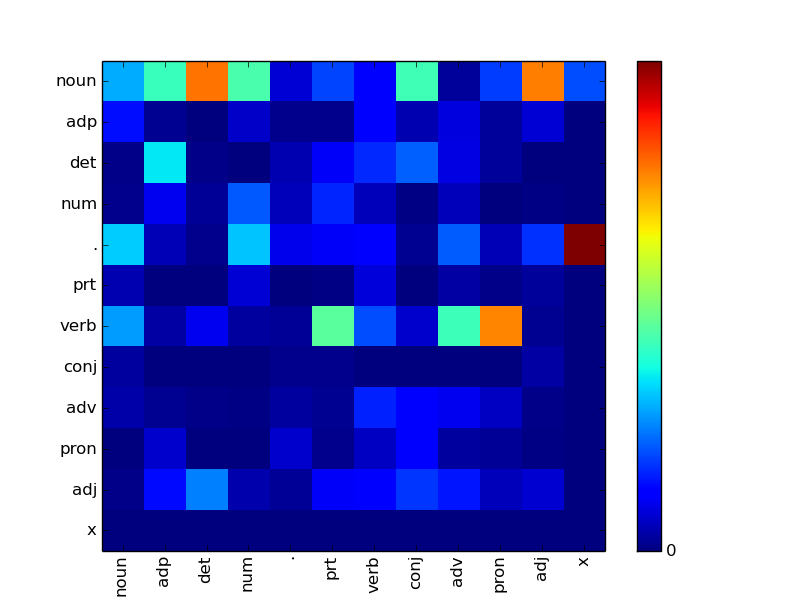
\includegraphics[scale=.5]{figs/sequences/transition_probs}
\caption{\label{fig:transProbs} Transition probabilities of the
trained model. Each column is the previous state and row is the current
state. Note the high probability of having Noun after Determinant or Adjective, or of having Verb after Nouns or Pronouns, as expected.}
\end{figure}

\begin{exercise}
Test the model using both posterior decoding and Viterbi decoding on
both the train and test set, using the methods in class HMM:
\begin{python}
>>> viterbi_pred_train = hmm.viterbi_decode_corpus(train_seq)
>>> posterior_pred_train = hmm.posterior_decode_corpus(train_seq)
>>> eval_viterbi_train =   hmm.evaluate_corpus(train_seq, viterbi_pred_train)
>>> eval_posterior_train =  hmm.evaluate_corpus(train_seq, posterior_pred_train)
>>> print "Train Set Accuracy: Posterior Decode \%.3f, Viterbi Decode: \%.3f"\%(eval_posterior_train,eval_viterbi_train)
Train Set Accuracy: Posterior Decode 0.985, Viterbi Decode: 0.985
>>> viterbi_pred_test = hmm.viterbi_decode_corpus(test_seq)
>>> posterior_pred_test = hmm.posterior_decode_corpus(test_seq)
>>> eval_viterbi_test =   hmm.evaluate_corpus(test_seq,viterbi_pred_test)
>>> eval_posterior_test = hmm.evaluate_corpus(test_seq,posterior_pred_test)
>>> print "Test Set Accuracy: Posterior Decode \%.3f, Viterbi Decode: \%.3f"\%(eval_posterior_test,eval_viterbi_test)
Test Set Accuracy: Posterior Decode 0.350, Viterbi Decode: 0.509
\end{python}
What do you observe? Remake the previous exercise but now train the HMM
using smoothing. Try different values (0,0.1,0.01,1) and report the results on the
train and development set. (Use function
\emph{pick\_best\_smoothing}).


\begin{python}
>>> best_smoothing = hmm.pick_best_smoothing(train_seq, dev_seq, [10,1,0.1,0])
Smoothing 10.000000 --  Train Set Accuracy: Posterior Decode 0.731, Viterbi Decode: 0.691
Smoothing 10.000000 -- Test Set Accuracy: Posterior Decode 0.712, Viterbi Decode: 0.675
Smoothing 1.000000 --  Train Set Accuracy: Posterior Decode 0.887, Viterbi Decode: 0.865
Smoothing 1.000000 -- Test Set Accuracy: Posterior Decode 0.818, Viterbi Decode: 0.792
Smoothing 0.100000 --  Train Set Accuracy: Posterior Decode 0.968, Viterbi Decode: 0.965
Smoothing 0.100000 -- Test Set Accuracy: Posterior Decode 0.851, Viterbi Decode: 0.842
Smoothing 0.000000 --  Train Set Accuracy: Posterior Decode 0.985, Viterbi Decode: 0.985
Smoothing 0.000000 -- Test Set Accuracy: Posterior Decode 0.370, Viterbi Decode: 0.526
>>> hmm.train_supervised(train_seq, smoothing=best_smoothing)
>>> viterbi_pred_test = hmm.viterbi_decode_corpus(test_seq)
>>> posterior_pred_test = hmm.posterior_decode_corpus(test_seq)
>>> eval_viterbi_test =   hmm.evaluate_corpus(test_seq, viterbi_pred_test)
>>> eval_posterior_test = hmm.evaluate_corpus(test_seq, posterior_pred_test)
>>> print "Best Smoothing \%f --  Test Set Accuracy: Posterior Decode \%.3f, Viterbi Decode: \%.3f"%(best_smoothing,eval_posterior_test,eval_viterbi_test)
Best Smoothing 0.100000 --  Test Set Accuracy: Posterior Decode 0.837, Viterbi Decode: 0.827
\end{python}


Perform some error analysis to understand were the errors are coming
from. You can start by visualizing the confusion matrix (true tags vs
predicted tags). You should get something like what is shown in Figure~\ref{fig:cmuns}.

\begin{python}
>>> import lxmls.sequences.confusion_matrix as cm
>>> import matplotlib.pyplot as plt
>>> confusion_matrix = cm.build_confusion_matrix(test_seq.seq_list, viterbi_pred_test, len(corpus.tag_dict), hmm.get_num_states())
>>> cm.plot_confusion_bar_graph(confusion_matrix, corpus.tag_dict, xrange(hmm.get_num_states()), 'Confusion matrix')
>>> plt.show()
\end{python}

\begin{figure}[h!]
\centering
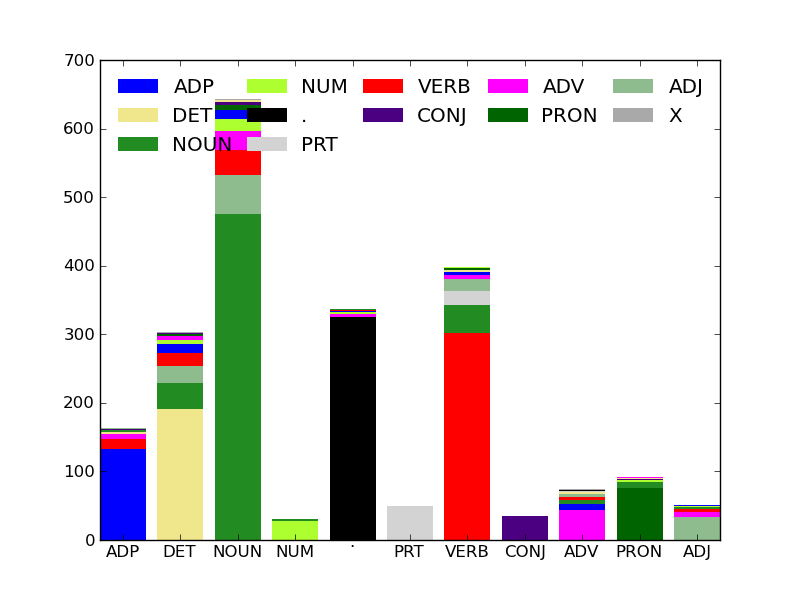
\includegraphics[scale=.4]{figs/sequences/cm_sup.png}
\caption{\label{fig:cmuns} Confusion Matrix for the previous
  example. Predicted tags are columns and the true tags corresponds to
  the constituents of each column.}
\end{figure}

\end{exercise}


%\begin{exercise}
%Implement a function that produces the accuracy for rare words vs
%common words. Use you own definition of rare word.
%
%Can you come up with other error analysis methods? Which?
%
%\end{exercise}

%\begin{exercise}
%So far we have only worked with a limited dataset of 1000 words. Try increasing the number of sentences to 10000. What do you observe?
%\end{exercise}


%\section{Unsupervised Learning of HMMs}
%
%\afm{explain here the EM algorithm}
%
%\begin{python}
%
%Initial accuracy: 0.303638
%Iter: 1 Log Likelihood: -101824.763927
%Iter: 1 Accuracy: 0.305441
%Iter: 2 Log Likelihood: -78057.108346
%Iter: 2 Accuracy: 0.321976
%Iter: 3 Log Likelihood: -77813.725501
%Iter: 3 Accuracy: 0.357451
%Iter: 4 Log Likelihood: -77192.947674
%Iter: 4 Accuracy: 0.385109
%Iter: 5 Log Likelihood: -76191.800849
%Iter: 5 Accuracy: 0.392123
%Iter: 6 Log Likelihood: -75242.572729
%Iter: 6 Accuracy: 0.391121
%Iter: 7 Log Likelihood: -74392.892496
%Iter: 7 Accuracy: 0.404249
%Iter: 8 Log Likelihood: -73357.542833
%Iter: 8 Accuracy: 0.399940
%Iter: 9 Log Likelihood: -72135.182778
%Iter: 9 Accuracy: 0.399238
%Iter: 10 Log Likelihood: -70924.246230
%Iter: 10 Accuracy: 0.395430
%Iter: 11 Log Likelihood: -69906.561800
%Iter: 11 Accuracy: 0.394328
%Iter: 12 Log Likelihood: -69140.228623
%Iter: 12 Accuracy: 0.390821
%Iter: 13 Log Likelihood: -68541.416423
%Iter: 13 Accuracy: 0.391522
%Iter: 14 Log Likelihood: -68053.456865
%Iter: 14 Accuracy: 0.389117
%Iter: 15 Log Likelihood: -67667.318961
%Iter: 15 Accuracy: 0.386411
%Iter: 16 Log Likelihood: -67337.685686
%Iter: 16 Accuracy: 0.385409
%Iter: 17 Log Likelihood: -67054.571821
%Iter: 17 Accuracy: 0.385409
%Iter: 18 Log Likelihood: -66769.973881
%Iter: 18 Accuracy: 0.385409
%Iter: 19 Log Likelihood: -66442.608458
%Iter: 19 Accuracy: 0.385409
%
%\end{python}
